\documentclass[11pt]{article}

\usepackage[margin=1in]{geometry}
\usepackage{graphicx}
\usepackage{booktabs}
\usepackage{amsmath}
\usepackage{amssymb}
\usepackage[round]{natbib}
\usepackage[hidelinks]{hyperref}

\graphicspath{{../figures/}}
\newcommand{\sampleStart}{December 2002}
\newcommand{\sampleEnd}{August 2018}
\newcommand{\nStocks}{100}
\newcommand{\nMonths}{189}
\newcommand{\momMean}{-0.45\%}
\newcommand{\momAnn}{-5.42\%}
\newcommand{\momVol}{30.42\%}
\newcommand{\momSharpe}{-0.18}
\newcommand{\momTnw}{-0.65}
\newcommand{\momMin}{-56.88\%}
\newcommand{\momMinMonth}{April 2009}
\newcommand{\momHit}{46.6\%}
\newcommand{\momCum}{-80.5\%}
\newcommand{\momMonths}{176}
\newcommand{\decLosers}{1.08\%}
\newcommand{\decWinners}{0.63\%}
\newcommand{\quintMean}{-0.23\%}
\newcommand{\quintTnw}{-0.46}
\newcommand{\capmAlpha}{-0.02\%}
\newcommand{\capmAlphaT}{-0.04}
\newcommand{\ffThreeAlpha}{-0.18\%}
\newcommand{\ffThreeAlphaT}{-0.33}
\newcommand{\ffFourAlpha}{-0.72\%}
\newcommand{\ffFourAlphaAnn}{-8.59\%}
\newcommand{\ffFourAlphaT}{-2.22}
\newcommand{\ffFourWmlBeta}{1.84}
\newcommand{\ffFourWmlT}{14.45}
\newcommand{\ffFourRsq}{0.70}
\newcommand{\umdCorr}{0.83}
\newcommand{\ivMean}{0.80\%}
\newcommand{\ivAnn}{9.56\%}
\newcommand{\ivSharpe}{0.78}
\newcommand{\ivTnw}{2.73}
\newcommand{\ivCum}{265\%}
\newcommand{\ewMean}{0.87\%}
\newcommand{\ewSharpe}{0.74}
\newcommand{\ewCum}{301\%}
\newcommand{\activeMean}{-0.07\%}
\newcommand{\activeTnw}{-1.04}
\newcommand{\activeAlpha}{0.01\%}
\newcommand{\activeAlphaT}{0.18}
\newcommand{\betaMktMean}{-0.06}
\newcommand{\betaSmbMean}{-0.08}
\newcommand{\betaHmlMean}{-0.05}
\newcommand{\rollRsq}{0.61}
\newcommand{\momTurnover}{115\%}
\newcommand{\ivTurnover}{7.9\%}
\newcommand{\ewTurnover}{4.5\%}
\newcommand{\momNetFifty}{-1.03\%}
\newcommand{\revMkt}{0.18}
\newcommand{\revSmb}{0.28}
\newcommand{\revHml}{0.73}


\setlength{\parskip}{0.5em}
\setlength{\parindent}{0pt}

\begin{document}

\begin{titlepage}
  \centering
  \vspace*{5cm}
  {\LARGE\bfseries US Equity Momentum and Inverse-Volatility Portfolios\par}
  \vspace{1.5cm}
  {\large David Dümig\par}
  \vfill
\end{titlepage}

\begin{abstract}
\noindent
This study rebuilds, from monthly prices of \nStocks{} US large-cap stocks between \sampleStart{}
and \sampleEnd{}, a decile momentum strategy and an inverse-volatility portfolio measured against
an equal-weight benchmark. Over this sample the momentum long-short lost \momMean{} per month and
is not statistically distinguishable from zero. It carries a large loading on the published
momentum factor yet a significant negative four-factor alpha, so a ten-percent breakpoint
equal-weighted construction is a weaker version of the factor. The inverse-volatility portfolio
tracked the equal-weight benchmark closely, with an active return that was small and
insignificant. The results survive alternative formation windows, quintile sorting, and
transaction costs.
\end{abstract}

\section{Introduction}

Momentum, the tendency of recent winners to keep outperforming recent losers, is one of the most
studied anomalies in asset pricing \citep{jegadeesh1993, carhart1997}. Risk-based weighting, which
tilts a portfolio toward lower-volatility names, is a common alternative to market-capitalisation
or equal weighting. This study examines both on a single panel of \nStocks{} US large-cap stocks.

Three questions are addressed. First, a momentum strategy is built by sorting stocks into deciles
on their past return and holding the top decile against the bottom decile. Second, an
inverse-volatility portfolio is compared with an equal-weight benchmark, and the active return
between them is decomposed with a rolling Fama-French regression. Third, a short identity for the
volatility contribution of a factor is derived. The headline finding is that momentum did not pay
in this sample: average returns are flat to slightly declining across the deciles, and the
long-short was driven deeply negative by the rebound of \momMinMonth{}, consistent with the
momentum crashes documented by \citet{daniel2016}.

\section{Data}

The universe is \nStocks{} US large-cap stocks. Monthly closing prices in US dollars, including
dividends, run from November 2002 to \sampleEnd{}, which gives \nMonths{} monthly returns from
\sampleStart{}. Returns are arithmetic, $r_{i,t} = P_{i,t}/P_{i,t-1} - 1$.

Factor returns are the Kenneth French North American market, size, and value factors, the
risk-free rate, and the North American momentum factor \citep{fama1993, fama2012, frenchdata}. The
series pasted into the original workbook are used for the replication, so the rebuilt numbers can
be checked against the original cell by cell. A script also downloads the current factor files and
records the download date in the repository. The current files differ from the 2018 copies by up
to \revHml{} percentage points on value, \revSmb{} on size, and \revMkt{} on the market in
individual months, which reflects the routine revisions Kenneth French applies to the North
American history; the risk-free rate is unchanged.

\section{Method}

\subsection{Momentum}

For each month the formation return is the twelve-month price change that skips the most recent
month, $F_{i,t} = P_{i,t-2}/P_{i,t-14} - 1$. The skip avoids the short-term reversal in the latest
month. Stocks are ranked on $F_{i,t}$ and split into ten deciles of ten stocks. Each decile return
is the equal-weight average of its stocks' returns in the holding month, and the strategy return is
the top decile minus the bottom decile.

\subsection{Inverse-volatility and equal-weight portfolios}

Each stock's volatility is the sample standard deviation of its returns over the trailing twelve
months, excluding the current month. The inverse-volatility weight is
$w_{i,t} = (1/\sigma_{i,t}) / \sum_j (1/\sigma_{j,t})$, and the portfolio return is
$\sum_i w_{i,t} r_{i,t}$. The equal-weight benchmark holds one percent in each stock. The active
return is the inverse-volatility return minus the equal-weight return.

\subsection{Rolling factor model}

The active return is regressed on the market, size, and value factors over a rolling twelve-month
window by ordinary least squares with an intercept. The estimated betas are applied to the current
month's factors to split the active return into a systematic part, $\alpha + \sum_k \beta_k f_{k,t}$,
and an idiosyncratic residual. Statistical significance uses Newey-West standard errors
\citep{newey1987}.

\subsection{A volatility contribution identity}

Writing a portfolio return as a sum of components $r_i = a_i + \beta_{i,p} f_i + \varepsilon_i$ and
using $\operatorname{cov}(X,Y) = \sigma(X)\,\sigma(Y)\,\operatorname{corr}(X,Y)$,
\begin{align}
\sigma^2(r_p) &= \operatorname{cov}\Big(r_p, \sum_{i=1}^N r_i\Big)
             = \sigma(r_p) \, \sigma\Big(\sum_i r_i\Big) \operatorname{corr}\Big(r_p, \sum_i r_i\Big).
\end{align}
Dividing by $\sigma(r_p)$ and expanding each component, the constant terms have zero volatility and
zero correlation with the portfolio, which leaves the contribution of each factor to portfolio
volatility,
\begin{align}
\sigma(r_p) &= \sum_{i=1}^N \beta_{i,p} \, \sigma(f_i) \, \operatorname{corr}(r_p, f_i).
\end{align}

\section{Results}

\subsection{Momentum}

The momentum long-short returned \momMean{} per month over \momMonths{} months, an annualised
\momAnn{} with volatility \momVol{}, so the Sharpe ratio is \momSharpe{}. The Newey-West
t-statistic is \momTnw{}, so the strategy is not distinguishable from zero. Average returns do not
rise across the deciles: the loser decile averaged \decLosers{} per month against \decWinners{} for
the winner decile (Figure~\ref{fig:deciles}). The worst month was \momMin{} in \momMinMonth{}, when
prior losers rebounded sharply, and the strategy's cumulative return over the sample was \momCum{}
(Figure~\ref{fig:momcum}). The strategy moves closely with the published momentum factor, with a
correlation of \umdCorr{} (Figure~\ref{fig:momumd}).

\begin{figure}[htbp]
  \centering
  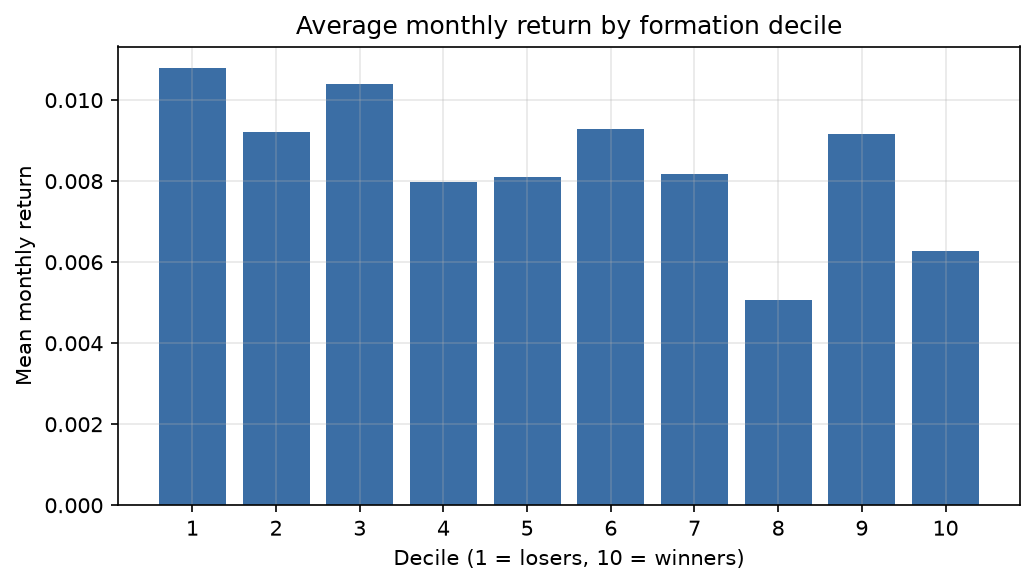
\includegraphics[width=0.78\linewidth]{decile_means.png}
  \caption{Average monthly return by formation decile. Decile 1 holds the lowest past returns and
  decile 10 the highest.}
  \label{fig:deciles}
\end{figure}

\begin{figure}[htbp]
  \centering
  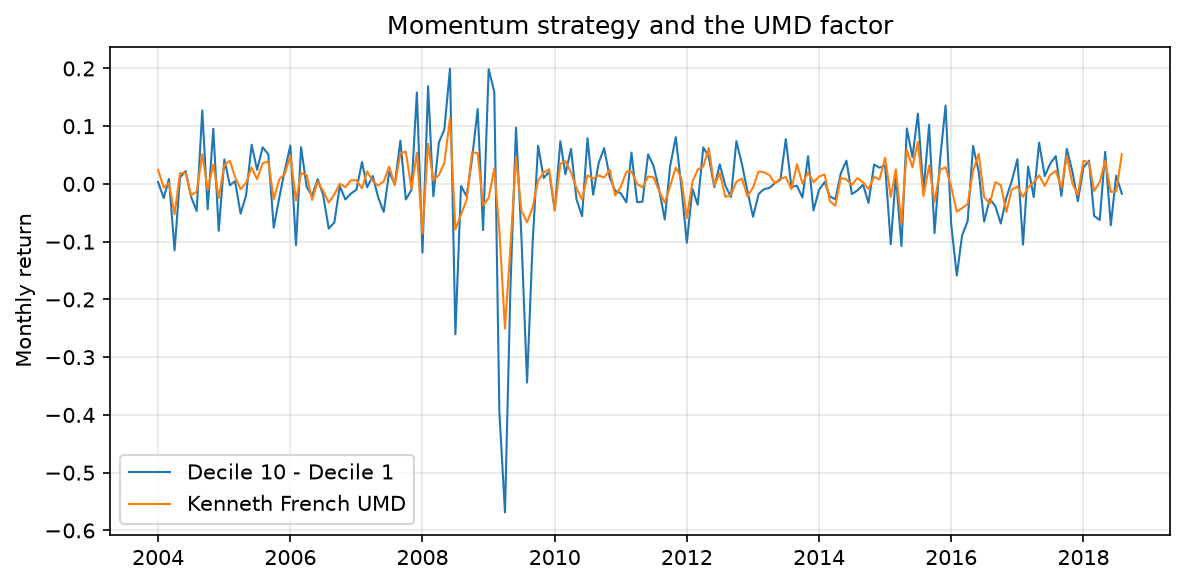
\includegraphics[width=0.9\linewidth]{momentum_vs_umd.png}
  \caption{The decile momentum long-short and the Kenneth French momentum factor.}
  \label{fig:momumd}
\end{figure}

\begin{figure}[htbp]
  \centering
  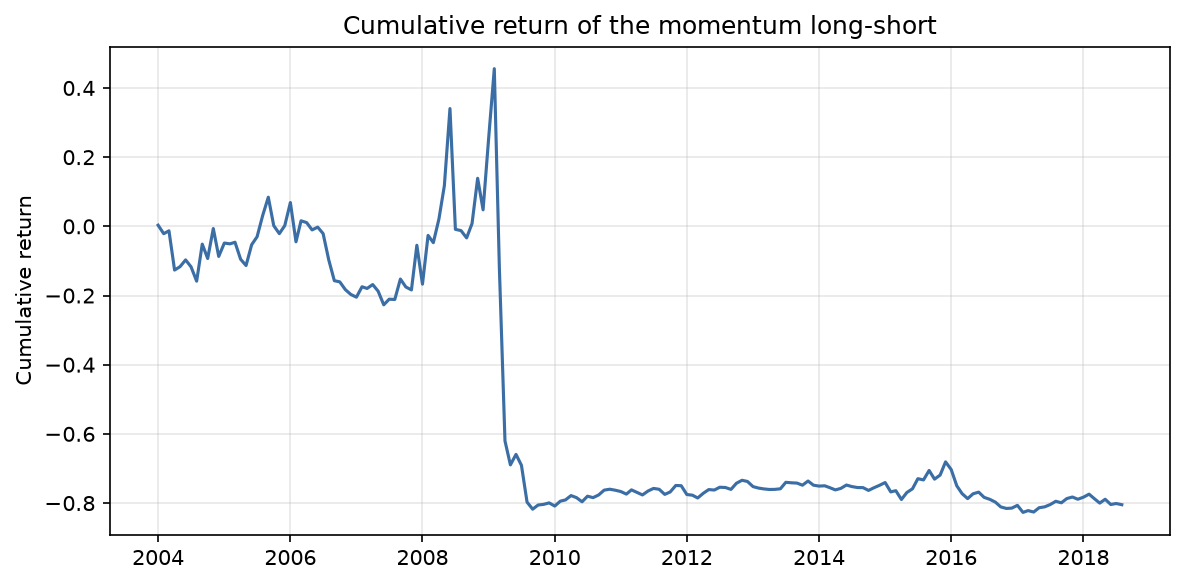
\includegraphics[width=0.82\linewidth]{momentum_cumulative.png}
  \caption{Cumulative return of the momentum long-short, including the \momMinMonth{} crash.}
  \label{fig:momcum}
\end{figure}

\subsection{Inverse-volatility and equal-weight portfolios}

The inverse-volatility portfolio returned \ivMean{} per month with a Sharpe ratio of \ivSharpe{},
close to the equal-weight benchmark at \ewMean{} and \ewSharpe{} (Table~\ref{tab:portfolio},
Figure~\ref{fig:ivew}). The active return was \activeMean{} per month with a Newey-West
t-statistic of \activeTnw{}, so the two portfolios are hard to tell apart. The rolling betas of the
active return move over time and average \betaMktMean{} on the market, \betaSmbMean{} on size, and
\betaHmlMean{} on value (Figure~\ref{fig:betas}). On average \rollRsq{} of the variance of the
active return is explained by the three factors, so a large part remains idiosyncratic
(Figures~\ref{fig:alpha} and~\ref{fig:sysidio}).

\begin{table}[htbp]
  \centering
  \caption{Portfolio statistics. Mean is per month, volatility is annualised, and the t-statistic
  uses Newey-West standard errors.}
  \label{tab:portfolio}
  \begin{tabular}{lccccc}
\toprule
Portfolio & Mean (mo) & Vol (yr) & Sharpe & NW $t$ & Cumulative \\
\midrule
Inverse volatility & 0.80\% & 12.21\% & 0.69 & 2.73 & 265\% \\
Equal weight & 0.87\% & 14.13\% & 0.66 & 2.53 & 301\% \\
Active (IV - EW) & -0.07\% & 2.97\% & -0.30 & -1.04 & -13\% \\
\bottomrule
\end{tabular}

\end{table}

\begin{figure}[htbp]
  \centering
  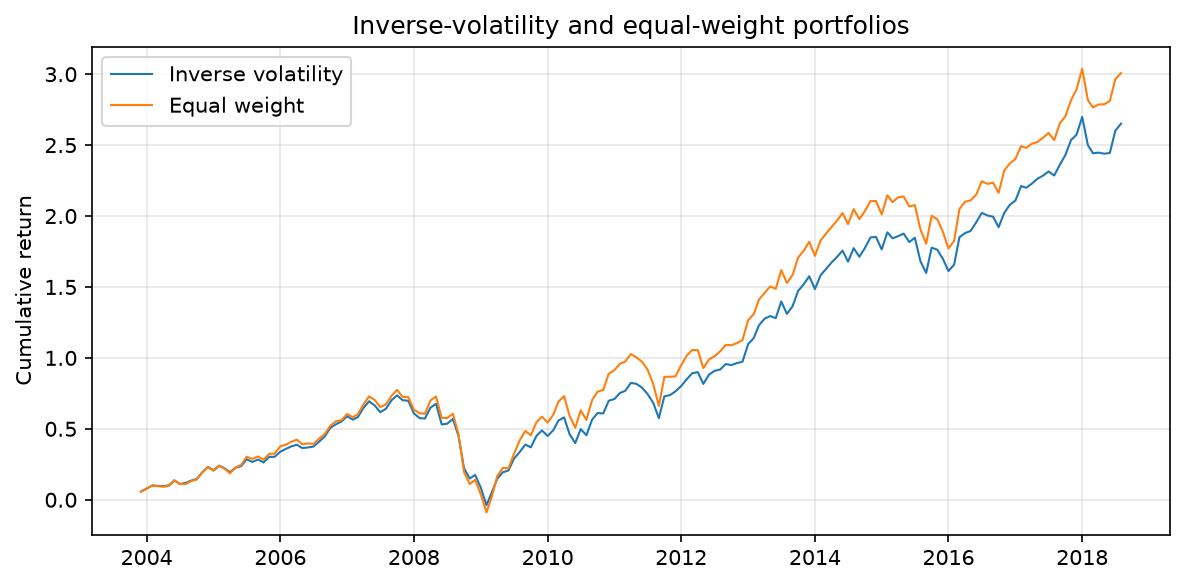
\includegraphics[width=0.82\linewidth]{iv_vs_ew_cumulative.png}
  \caption{Cumulative return of the inverse-volatility and equal-weight portfolios.}
  \label{fig:ivew}
\end{figure}

\begin{figure}[htbp]
  \centering
  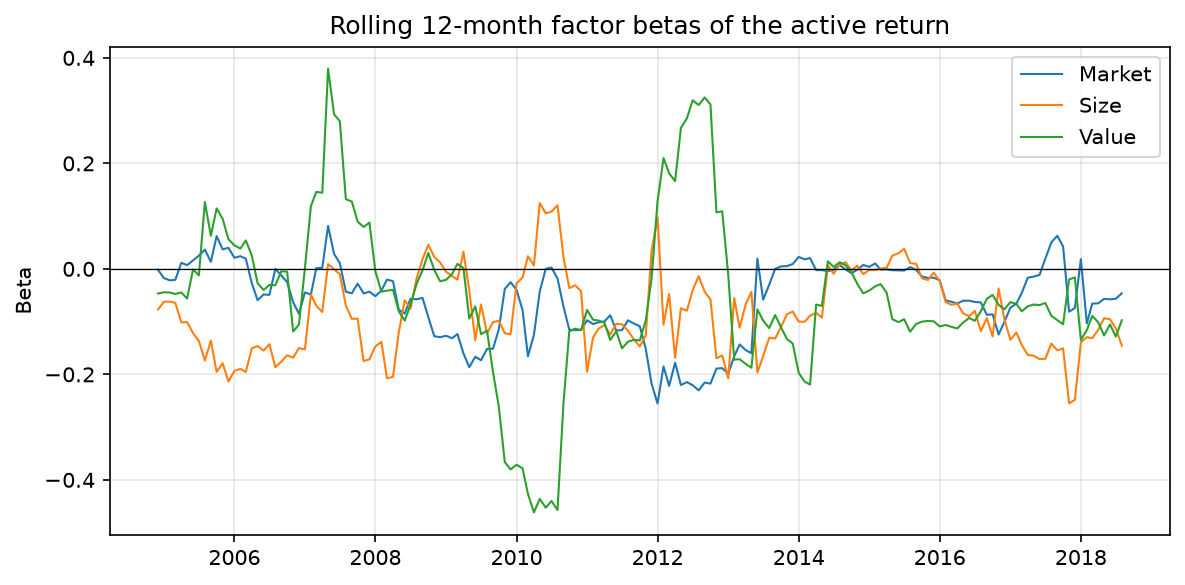
\includegraphics[width=0.9\linewidth]{rolling_betas.png}
  \caption{Rolling twelve-month factor betas of the active return.}
  \label{fig:betas}
\end{figure}

\begin{figure}[htbp]
  \centering
  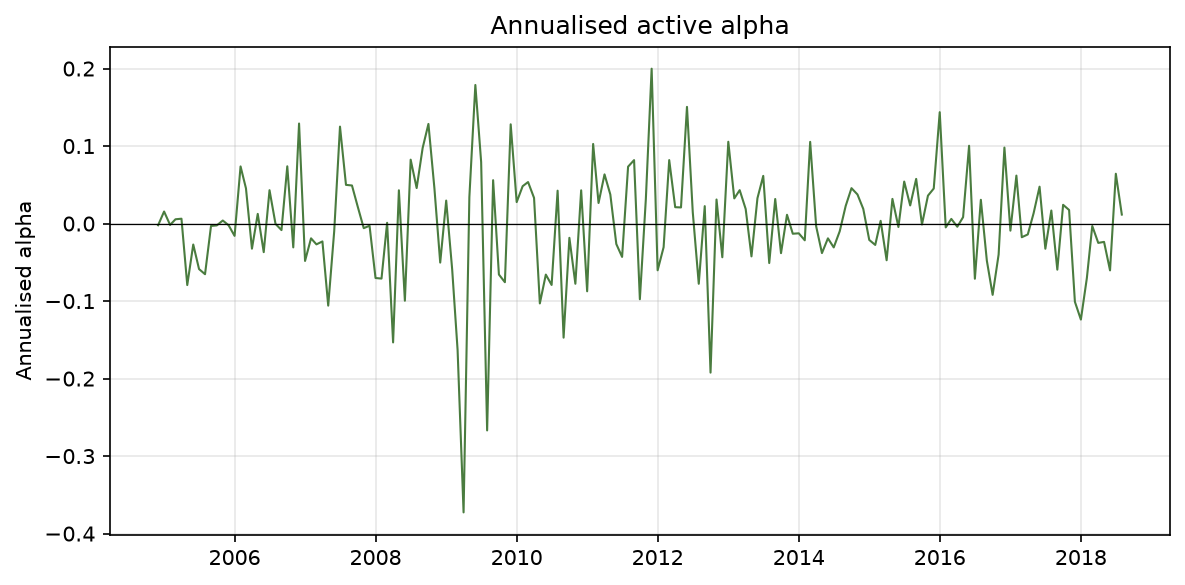
\includegraphics[width=0.82\linewidth]{annualised_alpha.png}
  \caption{Annualised active alpha from the rolling regression.}
  \label{fig:alpha}
\end{figure}

\begin{figure}[htbp]
  \centering
  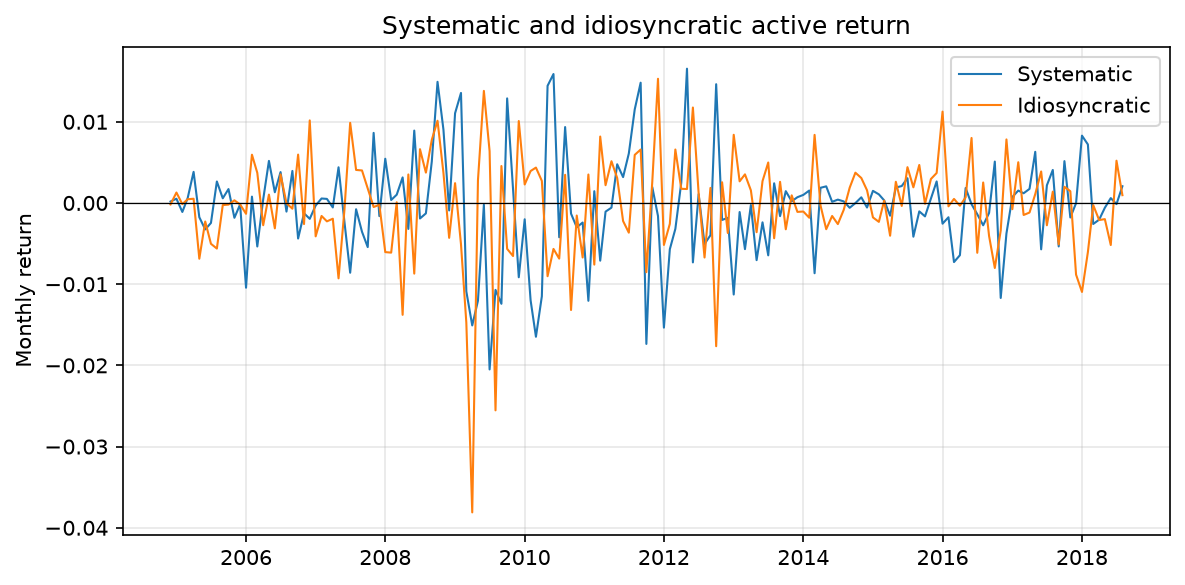
\includegraphics[width=0.9\linewidth]{systematic_idiosyncratic.png}
  \caption{Systematic and idiosyncratic parts of the active return.}
  \label{fig:sysidio}
\end{figure}

\section{Robustness}

\paragraph{Formation window.}
Three formation windows give the same message (Table~\ref{tab:formation}). Dropping the skip, or
shortening the window to six months, makes the long-short more negative, not less, so the
skip-month twelve-month definition is the least weak of the three and none of them pays.

\begin{table}[htbp]
  \centering
  \caption{Momentum long-short under alternative formation windows.}
  \label{tab:formation}
  \begin{tabular}{lcccc}
\toprule
Formation window & Months & Mean (per month) & NW $t$ & Sharpe \\
\midrule
12 months, skip most recent & 176 & -0.45\% & -0.65 & -0.18 \\
12 months, no skip & 177 & -0.55\% & -0.81 & -0.22 \\
6 months, skip most recent & 182 & -0.68\% & -1.10 & -0.30 \\
\bottomrule
\end{tabular}

\end{table}

\paragraph{Quintiles.}
With only \nStocks{} stocks, quintiles of twenty names are less noisy than deciles. The quintile
long-short returned \quintMean{} per month with a Newey-West t-statistic of \quintTnw{}, still
indistinguishable from zero.

\paragraph{Factor alphas.}
Table~\ref{tab:alphas} regresses the decile long-short on the CAPM, the Fama-French three-factor
model, and the Carhart four-factor model. The market and three-factor alphas are small and
insignificant. Under the four-factor model the strategy loads on the momentum factor with a beta of
\ffFourWmlBeta{} (t \ffFourWmlT{}), which lifts the fit to an $R^2$ of \ffFourRsq{}, yet the alpha
turns significantly negative at \ffFourAlpha{} per month (t \ffFourAlphaT{}). The decile long-short
is a weaker version of the published momentum factor, which uses wider breakpoints and value
weights.

\begin{table}[htbp]
  \centering
  \caption{Factor regressions of the momentum long-short. Alpha is per month; t-statistics use
  Newey-West standard errors.}
  \label{tab:alphas}
  \begin{tabular}{lccccccc}
\toprule
Model & $\alpha$ (mo) & $t(\alpha)$ & $\beta_{mkt}$ & $\beta_{smb}$ & $\beta_{hml}$ & $\beta_{umd}$ & $R^2$ \\
\midrule
CAPM & -0.02\% & -0.04 & -0.60 & -- & -- & -- & 0.07 \\
Fama-French 3 & -0.18\% & -0.33 & -0.55 & 0.28 & -1.32 & -- & 0.19 \\
Carhart 4 & -0.72\% & -2.22 & -0.26 & 0.16 & -0.19 & 1.84 & 0.70 \\
\bottomrule
\end{tabular}

\end{table}

\paragraph{Turnover and costs.}
The momentum long-short rebalances almost entirely each month, with two-way turnover of
\momTurnover{} per month, so costs matter: at fifty basis points per unit traded the mean return
falls to \momNetFifty{} per month (Table~\ref{tab:turnover}). The inverse-volatility and
equal-weight books trade far less, \ivTurnover{} and \ewTurnover{} per month, so costs barely move
the active return. The equal-weight benchmark still turns over because it is rebalanced back to
equal weights each month.

\begin{table}[htbp]
  \centering
  \caption{Two-way turnover and mean net return after costs, per month.}
  \label{tab:turnover}
  \begin{tabular}{lcccc}
\toprule
Book & Turnover (mo) & Net at 0 bps & Net at 10 bps & Net at 50 bps \\
\midrule
Momentum long-short & 115\% & -0.45\% & -0.57\% & -1.03\% \\
Active (IV - EW) & 7.9\% / 4.5\% & -0.07\% & -0.08\% & -0.09\% \\
\bottomrule
\end{tabular}

\end{table}

\paragraph{Replication.}
The Python rebuild matches the original workbook to floating-point precision across returns,
deciles, portfolios, and the rolling regression. One isolated error was found: in \momMinMonth's
neighbour month a formation-return tie placed one stock twice in a middle decile and dropped
another, which affected only that decile in that month and left the long-short unchanged. The
comparison is documented in the repository.

\section{Conclusion}

On this panel of \nStocks{} US large caps, momentum did not pay between \sampleStart{} and
\sampleEnd{}. The long-short was flat to negative, fragile to the \momMinMonth{} rebound, and
delivered a significant negative alpha once the momentum factor is included, which marks it as a
weaker version of the published factor rather than an independent source of return.
Inverse-volatility weighting produced almost the same result as equal weighting, with a small and
insignificant active return that the three factors explain only in part. The findings are stable
across formation windows, quintile sorting, and reasonable transaction costs.

\bibliographystyle{plainnat}
\bibliography{references}

\end{document}
